% 3 1 4 2
\documentclass{standalone}

\usepackage{tikz}
\usetikzlibrary{arrows.meta}

\begin{document}
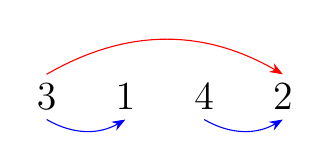
\begin{tikzpicture}[ele/.style = {font = \Large},
	inv/.style = {>=Stealth, ->, #1},]
  \foreach \e [count = \ei] in {3,1,4,2} {
	  \node (\e) [ele] at (\ei, 0) {$\e$};
  }

  \draw [inv = blue, bend right] (3.south) to (1.south);
  \draw [inv = red, bend left] (3.north) to (2.north);
  \draw [inv = blue, bend right] (4.south) to (2.south);
\end{tikzpicture}
\end{document}
